% Preambulo del documento
\documentclass[12pt, letterpaper]{article}

\usepackage{lipsum}
\usepackage[utf8]{inputenc}
\usepackage[dvipsnames]{xcolor}
\usepackage{graphicx}
\usepackage[spanish]{babel}
\usepackage{enumitem}
\usepackage{amsmath}

\graphicspath{{images/}}

\title{Primera sesión en LaTeX}
\author{Ronaldo Nolasco, Manuel Loaiza}
\date{\today}

\definecolor{micolor}{RGB}{0,255,255}

% Cuerpo del documento
\begin{document}
\maketitle
\tableofcontents
\pagebreak

\begin{abstract}
    El presente documento contiene todo lo desarrollado para la primera sesión del taller de LaTeX
\end{abstract}
\pagebreak

\section{LaTeX basico}

\subsection{Cuerpo del documento}

\lipsum[2-3]\newline
El texto de arriba es un texto de prueba.\\
Saldo de linea sin generar otro parrafo.

Mi primera sesión en LaTeX.

Mi batería está en un 75\%

\$ \&

\LaTeX\\

\subsection{Formato de texto}
%Formato de texto
Texto en \textbf{negrita}.\\
Texto en \textit{cursiva}.\\
Texto en \underline{subrayado}.\\
Texto en \emph{cursiva}.\\
\textit{\emph{T sobre E}}.\\
\emph{\textit{T sobre E}}.\\
Probando el color \textcolor{Red}{rojo}.\\
Probando el color de relleno \colorbox{Green}{verde}.\\
Probando el color personalizado \textcolor{micolor}{celeste}.\\
{\color{micolor}\rule{\linewidth}{1.5mm}}\\

\subsection{Imagenes y figuras}
%Imagenes en LaTeX
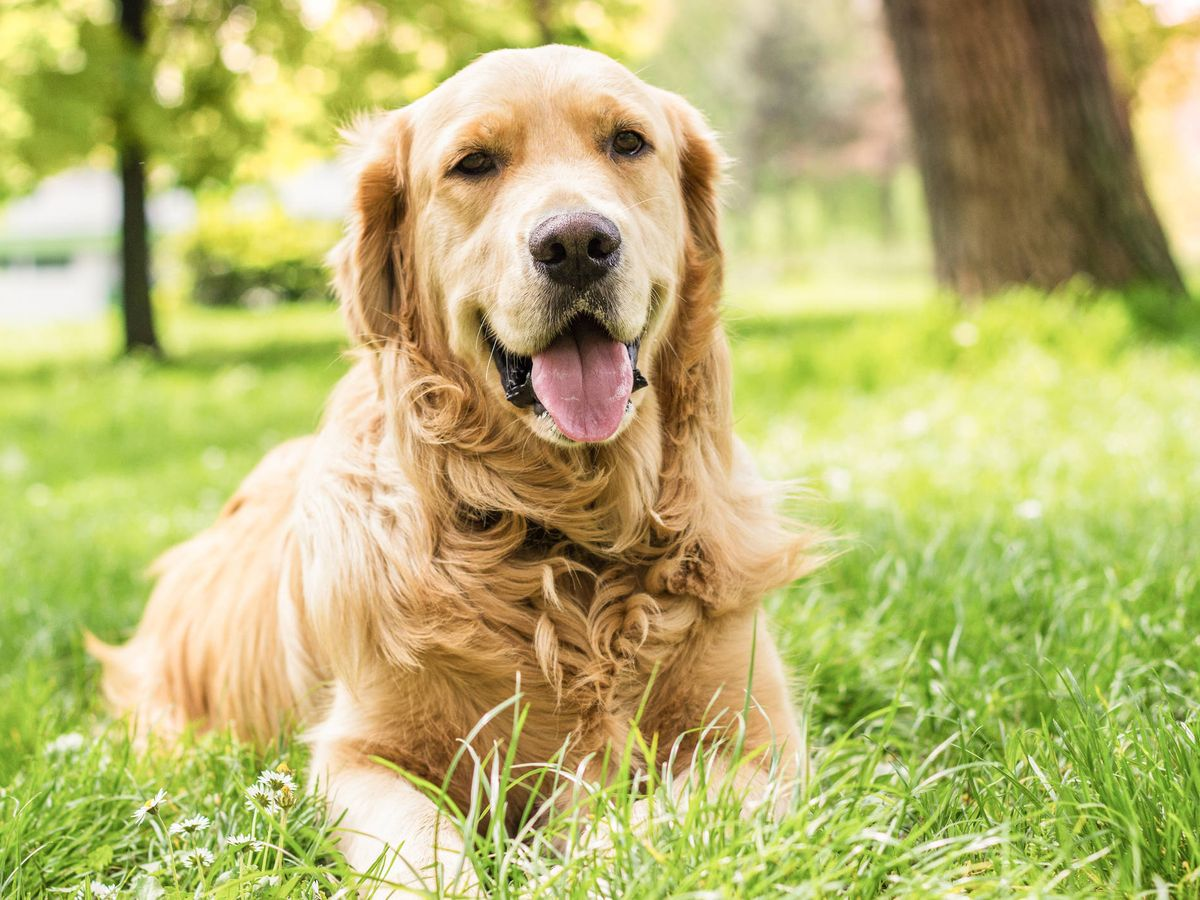
\includegraphics[height=4cm]{perro.jpg}

\begin{figure}[h]
    \centering
    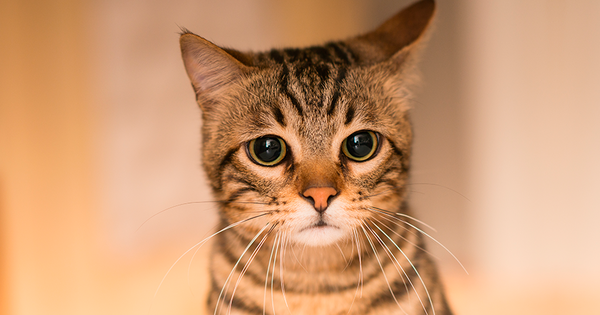
\includegraphics[height=4.5cm]{gato.png}
    \caption{Gato}
    \label{fig:gato}
\end{figure}

Hay un gatito en la figura \ref{fig:gato}.\\

\subsection{Listas y enumeraciones}
%Listas y enumeraciones
Mi lista de mascotas:
\begin{itemize}
    %\setlength\itemsep{3em}
    \item gato
    \item perro
    \item hamster
    \item pajaro
    \item pez\\
\end{itemize}

Mi lista de tareas:
\begin{enumerate}[noitemsep, nolistsep]
    \item Levantarme todos los días a las 6am.
    \item Salir a correr a las 7am.
    \item Alistarme para el trabajo a las 9am.
    \item Alistarme para las clases a las 4pm.
    \item Dormir a las 11pm.\\
\end{enumerate}

\section{LaTeX intermedio}
\subsection{Expresiones y formulas matemáticas}
%Expresiones y formulas matemáticas
La relación entre masa y energía es $E = mc^2$\\

El teorema de Pitágoras es: $$a^2 + b^2 = c^2$$

\begin{equation}
    \alpha + 2\beta = 50
\end{equation}
\begin{equation}
    3\alpha - \beta = 45
\end{equation}
De (1) y (2):
\begin{equation*}
    \boxed{\alpha = 20 \wedge \beta = 15}
\end{equation*}
%\[\alpha = 20 \wedge \beta = 15\]

\begin{align*}
    f(x) &= x^2\\
    g(x) &= \frac{1}{x}\\
    h(x) &= \int^a_b \frac{1}{3}x^3\\
\end{align*}

\subsection{Tablas}
%\begin{table}
\begin{center}
    \begin{tabular}{|c|c|c|c|}
        \hline
        \textbf{ID} & \textbf{Nombre} & \textbf{Telefono} & \textbf{Nacionalidad}\\
        \hline
        1 & Franz Bendezu & 912314664 & Peruano\\
        \hline
        2 & Manuel Loaiza & 946464465 & Colombiano\\
        \hline
        3 & Misael Abanto & 943311334 & Venezolano\\
        \hline
    \end{tabular}
\end{center}

\end{document}
